\documentclass[main.tex]{subfiles}
\section{The Van der Pol System}
In this section we are going to test the implemented methods using the Van der Pol oscillator. This particular initial value problem is very useful to evaluate how numerical solvers respond to stiffness.

Intuitively one can think of stiff problems as those whose solution varies rapidly in a short time span. This characteristic has an strong impact in some numerical methods that might need to take very small steps to get an accurate solution. Since their approximation is based in previous points, explicit methods are specially affected by this phenomena. For these methods, spontaneous variations have an strong effect on the truncation errors and make the numerical solution diverge from the real one. The concept of stiffness is strongly related to the stability of numerical algorithms which is discussed in sections 3 and 5.

Figure \ref{fig:VanderPolmu3} shows the solution obtained with the 5 different methods when $\mu = 3$. The graph on the left is the error estimation. In this case, all methods are able to converge to the true solution without having to take very small steps.

\begin{figure}[H]
    \centering
    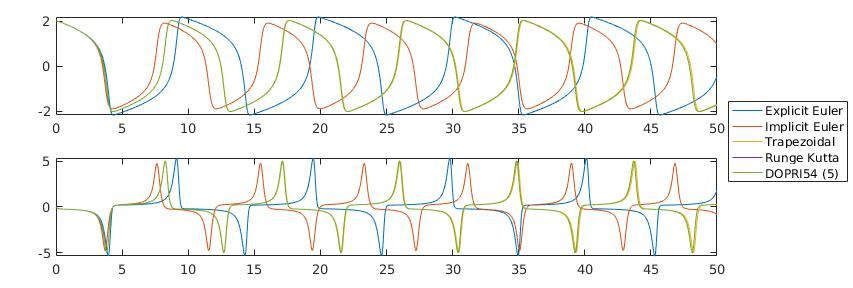
\includegraphics[width=\textwidth,clip]{../Figures/VanderPolmu3}
    \caption{Van der Pol oscillator solution from $t = 0$ to $t = 50$ for $\mu = 3$ and $h = 0.05$}
    \label{fig:VanderPolmu3}
\end{figure}

On the other hand, figure \ref{fig:VanderPolmu100} shows the solution for $\mu = 100$. For this value of the parameter the problem becomes very stiff in some regions. The bottom graph represents the degree of variation and the peaks give a measure of how fast the solution moves. We see that while the explicit algorithms are unable to handle the problem and their error blows up, implicit methods such as backward Euler can easily follow the solution track because the rely on future values and thus, they are aware in advance of those rapid variations.


\begin{figure}[H]
    \centering
    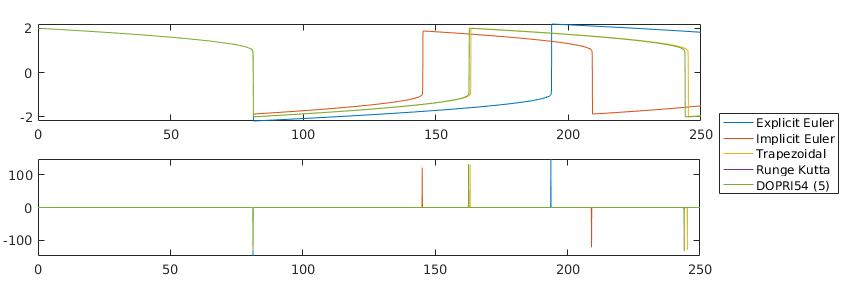
\includegraphics[width=\textwidth,clip]{../Figures/VanderPolmu100}
    \caption{Van der Pol oscillator solution from $t = 0$ to $t = 250$ for $\mu = 100$ and $h = 0.0025$}
    \label{fig:VanderPolmu100}
\end{figure}

We have measured the local error at $t = t_0 + h$ for different step sizes and $\mu = 100$. Figure \ref{fig:VanderPolError} shows that the implicit methods, that is, Implicit Euler and trapezoidal are accurate even when taking large steps. On the other hand, the error of the high order explicit methods becomes extremely large for step sizes of $10^-1$. The fact that the trapezoidal method is an hybrid of the forward and the backward finite difference approximations explains why implicit Euler performs better for large steps. 

\begin{figure}[H]
    \centering
    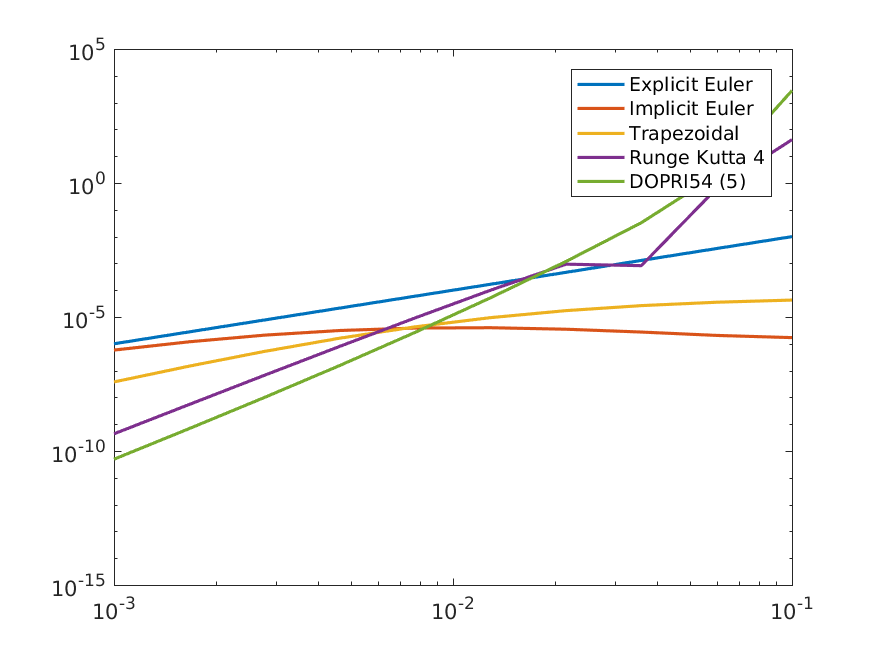
\includegraphics[width=\textwidth,clip]{../Figures/VanderPolError}
    \caption{Van der Pol oscillator local error estimates for $\mu = 100$}
    \label{fig:VanderPolError}
\end{figure}